%===============================================================================
% !TeX encoding = UTF-8
% !TeX spellcheck = ru_RU-Russian
% !TEX TS-program = latexmk
\documentclass[12pt,compress,aspectratio=169]{beamer}
%\documentclass[12pt,compress]{beamer}
%===============================================================================
\usepackage{mathtools}
\usepackage{amsmath}
\usepackage{amssymb}
\usepackage{bm}
\usepackage{tabularx}
\usepackage{multirow}
\usepackage{multicol}
\usepackage{nicefrac}
\usepackage{siunitx}
\usepackage{blindtext}

\graphicspath{{./pdf/}{./png/}{../Figures/}{./pics/}}
\usepackage[inkscapelatex=false]{svg}
\svgpath{{svg/}{../Figures/}}

% \usetheme{moloch}
% \usetheme{metropolis}
\usefonttheme[onlymath]{serif}

\usepackage{FiraSans}

% \usepackage[russian,english]{babel}
\usepackage[english,main=russian]{babel}  % https://tex.stackexchange.com/questions/86078/strange-latex-compilation-errors-triggered-by-the-number-of-lines-on-the-page

%\usepackage[]{plex-sans}
% \usetheme[progressbar=frametitle]{metropolis}
%\usetheme[progressbar=frametitle]{moloch}
\usetheme{moloch}
% 

% \setsansfont[ItalicFont={Fira Sans Light Italic},%
%                  BoldFont={Fira Sans SemiBold},%
%                  BoldItalicFont={Fira Sans Italic}]%
%                 {Fira Sans Light}%

\usepackage{appendixnumberbeamer}
\usepackage{booktabs}
\usepackage[scale=2]{ccicons}
\usepackage{pgfplots}
\usepgfplotslibrary{dateplot}

\usepackage{xspace}
% \newcommand{\themename}{\textbf{\textsc{metropolis}}\xspace}

\usepackage{fancyvrb}
\usepackage{minted}
% \usepackage{enumerate}
%\usepackage{metropolisbsuir} % Don't forget to load this!
\usepackage{molochbsuir} % Don't forget to load this!
\usepackage{tikz}

\usepackage[style=verbose,backend=biber]{biblatex}
\addbibresource{my_ref.bib}

%===============================================================================
%===============================================================================
%\setbeamersize{text margin left=5pt,text margin right=5pt}
%===============================================================================
%\usecolortheme{seahorse}

%\makeatletter
%\setlength{\metropolis@titleseparator@linewidth}{1pt}
%\setlength{\metropolis@progressonsectionpage@linewidth}{4pt}
%\setlength{\metropolis@progressinheadfoot@linewidth}{1pt}
%\makeatother

%\newcommand{\themename}{\textbf{\textsc{metropolis}}\xspace}

\makeatletter
\setbeamertemplate{title page}{
  \begin{minipage}[b]{\textwidth}
    \vfill%
    \ifx\inserttitle\@empty\else\usebeamertemplate*{title}\fi
    \ifx\insertsubtitle\@empty\else\usebeamertemplate*{subtitle}\fi
    \usebeamertemplate*{title separator}
    \ifx\beamer@shortauthor\@empty\else\usebeamertemplate*{author}\fi
    %\vspace{0.5cm} 
  \end{minipage}
  \vfil
  \begin{minipage}[t]{.58\textwidth}
    \vfill%
    \ifx\insertinstitute\@empty\else\usebeamertemplate*{institute}\fi
  \end{minipage}
  %\hfill
  \begin{minipage}[t]{.38\textwidth}
    \vfill
    \ifx\inserttitlegraphic\@empty\else\inserttitlegraphic\fi
  \end{minipage}
  \vfil
  \vspace{10pt}
  \ifx\insertdate\@empty\else\usebeamertemplate{date}\fi
}
\makeatother

\title{%
FPGA реализация нейронной сети прямого распространения для распознавания рукописных чисел}%
%\subtitle{ }
\date{ \tiny 20 ноября, 2024}
\author{{\bfseries Е.А. Кривальцевич}	\and М.И. Вашкевич \\ \texttt{ \footnotesize krivalcevi4.egor@gmail.com,\,\, vashkevich@bsuir.by}}
\institute{
  Белорусский государственный университет\\
  информатики и радиоэлектроники \\
  Кафедра электронных вычислительных средств \\
  \\
  \\
  XIV Международная научная конференции \\
  «Информационные технологии и системы»\\
  Минск, Республика Беларусь
}
\titlegraphic{
    
\includegraphics[height=1.3cm]{bsuir-logo.pdf} \\ \vspace{5pt} \\
    
\includegraphics[height=1.3cm]{its_logo.jpg}
}

\newcommand{\diag}[1]{	\operatorname{diag} \left( {#1} \right)	}
\newcommand{\ndiag}[1]{	\operatorname{diag} \left\lbrace {#1} \right\rbrace}
\newcommand{\bdiag}[1]{	\operatorname{diag} \left[ {#1} \right]}
\newcommand{\mtinyidx}[1]{	\textsc{\tiny \textit{#1}}}
\providecommand{\abs}[1]{\lvert#1\rvert}
\providecommand{\norm}[1]{\lVert#1\rVert}
\newcommand{\db}[1]{\SI{#1}{\decibel}}
\newcommand{\dbn}[1]{\SI{#1}{}}
\setbeamersize{text margin left=5pt,text margin right=5pt}

\begin{document}

\maketitle
%------------------------------------------------------------------------------------------
%===============================================================================
\begin{frame}
\frametitle{Содержание}

\begin{enumerate}
    \item Прототипирование нейронных сетей на FPGA 
    \item Постановка задачи
    \item Обучение нейронной сети
    \item Аппаратная реализация нейронной сети
    \item Использование PYNQ для прототипирования и тестирования нейронной сети
    \item Описание эксперимента и результаты
\end{enumerate}

\end{frame}
%===============================================================================


\section{Введение}
%===============================================================================
\begin{frame}
\frametitle{Прототипирование нейронных сетей на FPGA}
% \begin{columns}[T]
    % \column{0.7\textwidth}

    \begin{itemize}
        \item Вычислительной платформой для обучения и
        эксплуатации нейросетевых моделей чаще всего выступают графические процессоры,
        которые содержат множество вычислительных ядер, способных обрабатывать потоки данных
        параллельно. 
        \item FPGA (Field Programmable Gate Array) представляют собой реконфигурируемые вычислительные
        платформы, позволяющие реализовывать параллельно-поточные архитектуры НС.
        \item При реализации НС на базе FPGA появляется
        возможность использовать для представления параметров НС типов данных, обеспечивающих
        различную точность.
    \end{itemize}

    % \column{0.3\textwidth}
    % \begin{block}{\centering}
    %     \vspace{1mm}
    %     \centering
    %     \includesvg[height = 0.5\textheight]{RGB_multidim_data.svg}        
    % \end{block}
% \end{columns}
\end{frame}
%===============================================================================

\begin{frame}
\frametitle{Постановка задачи}

\begin{block}{\centering Цель исследования}                
    \begin{itemize}\small
        \item Получить аппаратно реализованную НС прямого распространения для распознавания рукописных цифр
        \item Выяснить влияние разрядности представления весовых коэффициентов НС на точность определения цифр и аппаратные затрат
        \item Оценить наиболее оптимальную реализацию НС           
    \end{itemize}
\end{block}
\end{frame}
%===============================================================================
\section{Обучение нейронной сети}
%===============================================================================
\begin{frame}
\frametitle{Архитектура нейронной сети}
\begin{columns}[T]
    \column{1\textwidth}
    
    \begin{block}{\centering Архитектура НС}
        \vspace{1mm}
        \centering 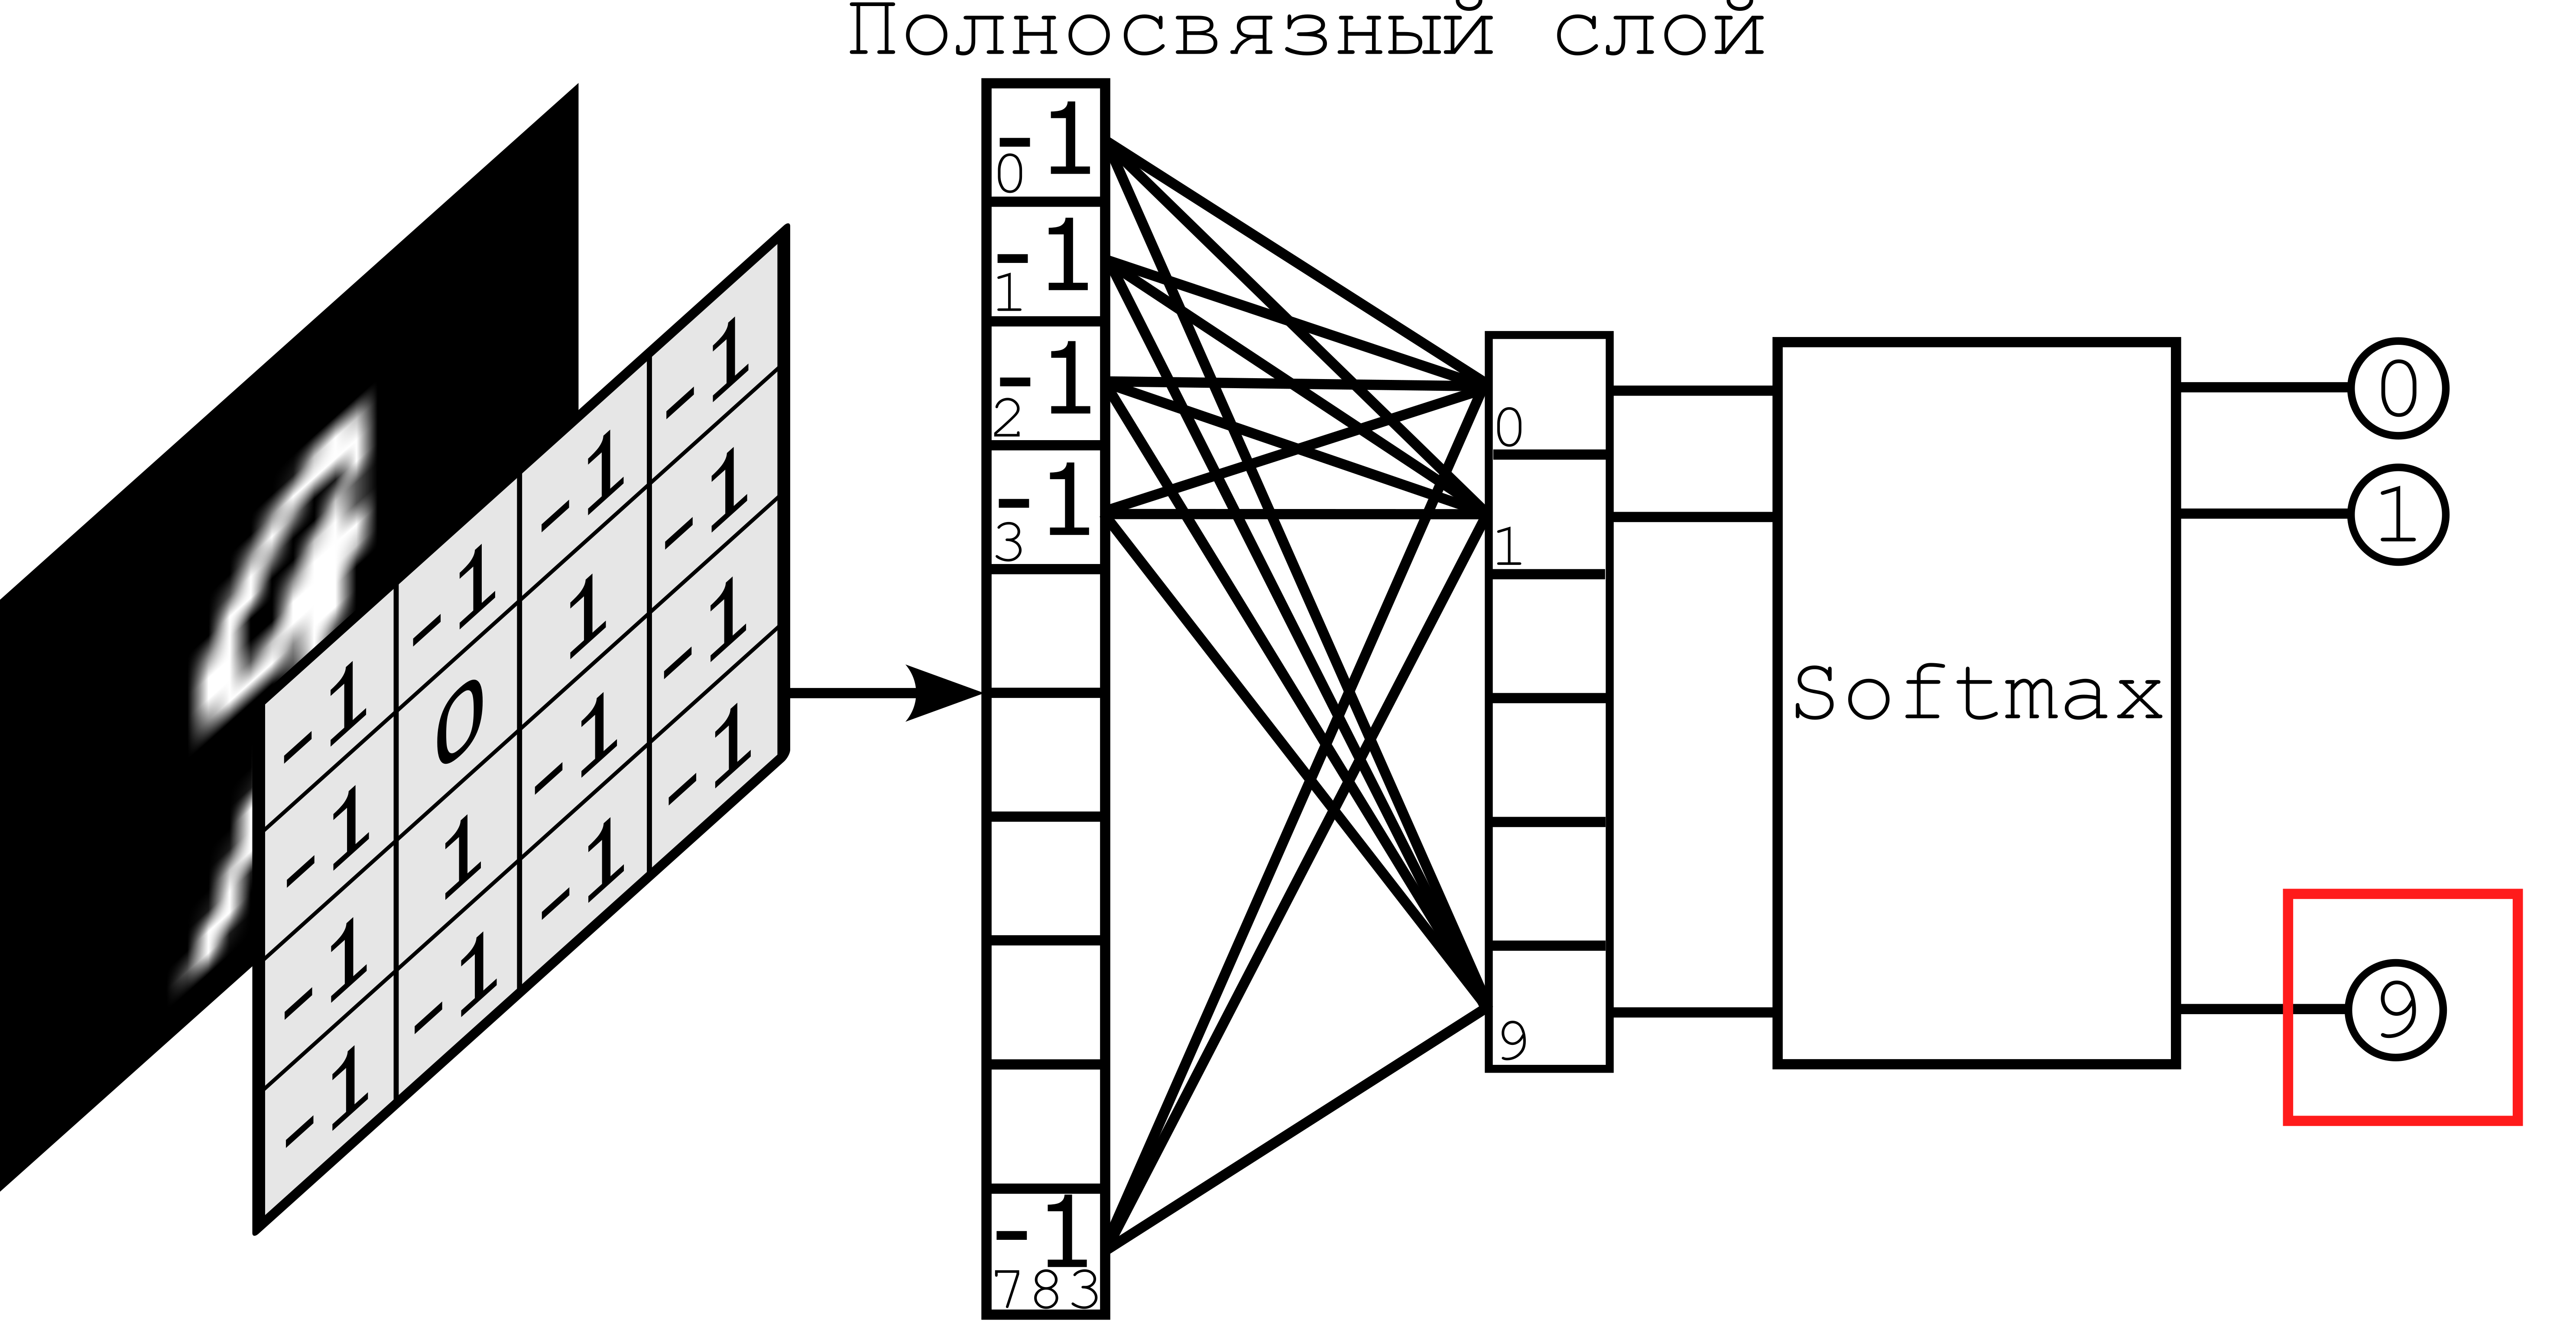
\includegraphics[width = 0.7\textwidth]{pics/nn.png}
        % \includesvg[height = 0.4\textheight]{basic_AE.svg}        
    \end{block}        

    \column{1\textwidth}
    \vspace{-2mm}
        
\end{columns}
\end{frame}
%===============================================================================
\begin{frame}[t]
    \frametitle{Параметры НС}
    \begin{itemize}
        \item Входные данные приводятся к диапазону [-1, 1] и устанавливается их
        среднеквадратическое отклонение(СКО) равным 0,5
        \item Оптимизация производилось с использованием метода стохастического градиентного спуска (SGD)
        (скорость обучения $\eta =3 \cdot 10^{-3}$, число эпох -- 10000, моментум $\gamma = 0,9$)
        \item Для оценки качества декодирования изображений использовались 
        метрика $MSE$
    \end{itemize}
    
    \end{frame}
    
\section{Аппаратная реализация нейронной сети}
%===============================================================================
\begin{frame}[t]
\frametitle{Аппаратная реализация нейронной сети}
\begin{block}{\centering Основные блоки}                
    \begin{itemize}\small
        \item Register file
        \item Counter
        \item Fully connected layer
        \item Max ind           
    \end{itemize}
\end{block}
\end{frame}
%===============================================================================
\begin{frame}[t]
    \frametitle{Структурная схема IP-блока}
    \begin{block}{}
        \vspace{1mm}
        \centering \includegraphics[height = 0.75\textheight]{pics/ip.png}
        % \includesvg[height = 0.4\textheight]{basic_AE.svg}        
    \end{block}   
\end{frame}

%===============================================================================


\section{Использование PYNQ для прототипирования и тестирования нейронной сети}
%===============================================================================
\begin{frame}[t]
    \frametitle{Структурная схема проекта}
    \begin{block}{} %{\centering Архитектура проекта}
        \vspace{1mm}
        \centering 
\includegraphics[width = 0.9\textwidth]{pics/struct_2.png}
        % \includesvg[height = 0.4\textheight]{basic_AE.svg}    
        \begin{itemize}\small
            \item Подключение PL блока к PS осуществляется с помощью AXI4-Lite и uP интерфейсов.
        \end{itemize}     
    \end{block}  
\end{frame}
%===============================================================================

% \begin{frame}[t]
% \frametitle{Автокодировщик на основе кватернионной НС}

% \begin{block}{\centering QAE -- \emph{quaternion autoencoder}}
%     \centering
% % \includesvg[height = 0.72\textheight]{QAE_scheme_ready.svg} 
% \end{block}
% \end{frame}
%===============================================================================
\section{Эксперимент и результаты}
%===============================================================================
\begin{frame}[t]
\frametitle{Описание эксперимента}
\begin{itemize}
    \item Набор данных MNSIT (10 тыс. изображений рукописных цифр $28 \times 28$)
    \item Данные подаются последовательно из процессорной системы
    \item Результаты группируются в виде матриц спутывания
    \item Проведено 15 тестов с различными разрядностями весовых коэффициентов (от 2 до 16)
    \item Составлен график зависимости точности от разрядности
    \item Разложены классы весовых коэффициентов на битовые плоскости
    \item Проанализированы аппаратные затраты
\end{itemize}

\end{frame}

%===============================================================================
\begin{frame}[t]
\frametitle{Результаты}
\begin{columns}
% \hspace{5mm}
\column[t]{0.45\textwidth}
% \begin{center}
\begin{block}{ \centering Матрица спутывания}
    \vspace{3mm}
    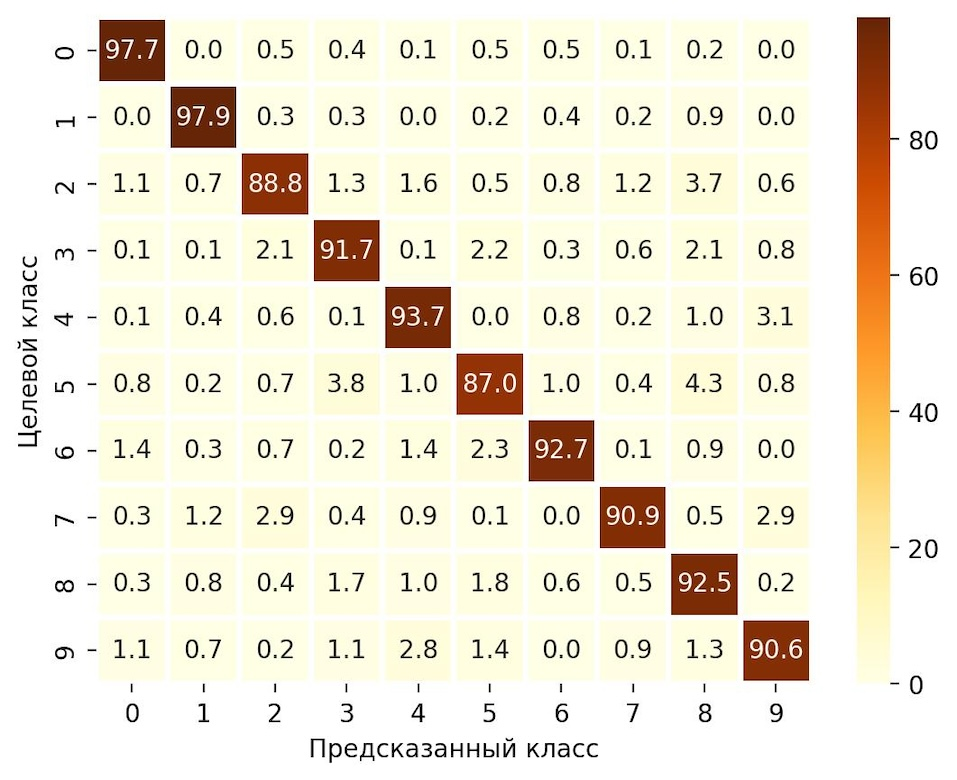
\includegraphics[width = 0.815\textwidth]{pics/cm_6q5.jpg} 
\end{block}
% \end{center}
 
\column[t]{0.45\textwidth}
\begin{block}{\centering Точность и затраты блоков LUT/FF}
    \vspace{3mm}
    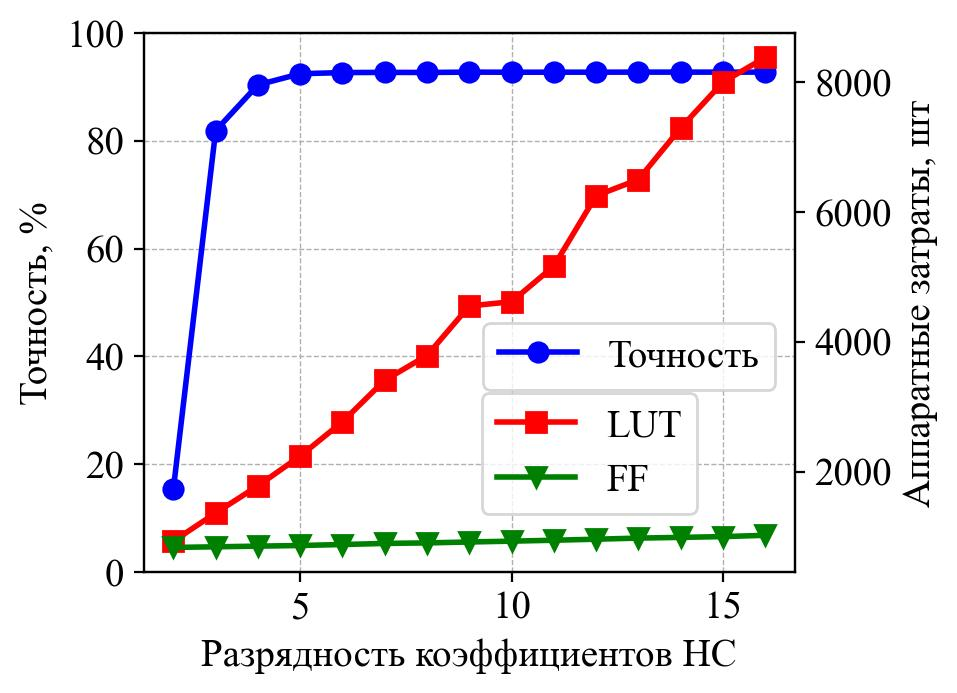
\includegraphics[width = 0.9\textwidth]{pics/Acc_LUTs_FFs.jpg} 
\end{block}

\end{columns}
\end{frame}

%===============================================================================
\begin{frame}[t]
\frametitle{Разложение на битовые плоскости}
\begin{columns}
    \hspace{5mm}
    \column[t]{0.3\textwidth}
    \centering 
    \begin{block}{\centering{Весовой класс 3}}
        \vspace{3mm}
        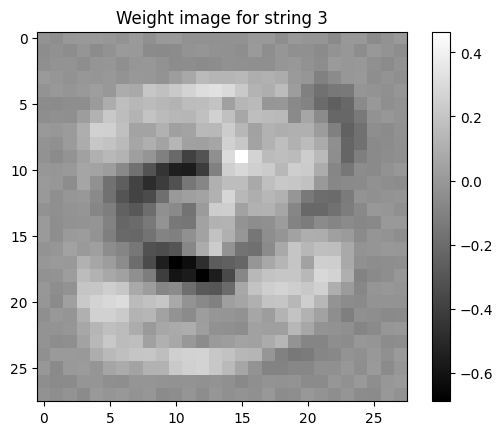
\includegraphics[width = 0.85\textwidth]{pics/output1.png} 
    \end{block}
     
    \column[t]{0.7\textwidth}
    \centering 
    \begin{block}{\centering{Битовые плоскости}}
        \vspace{3mm}
        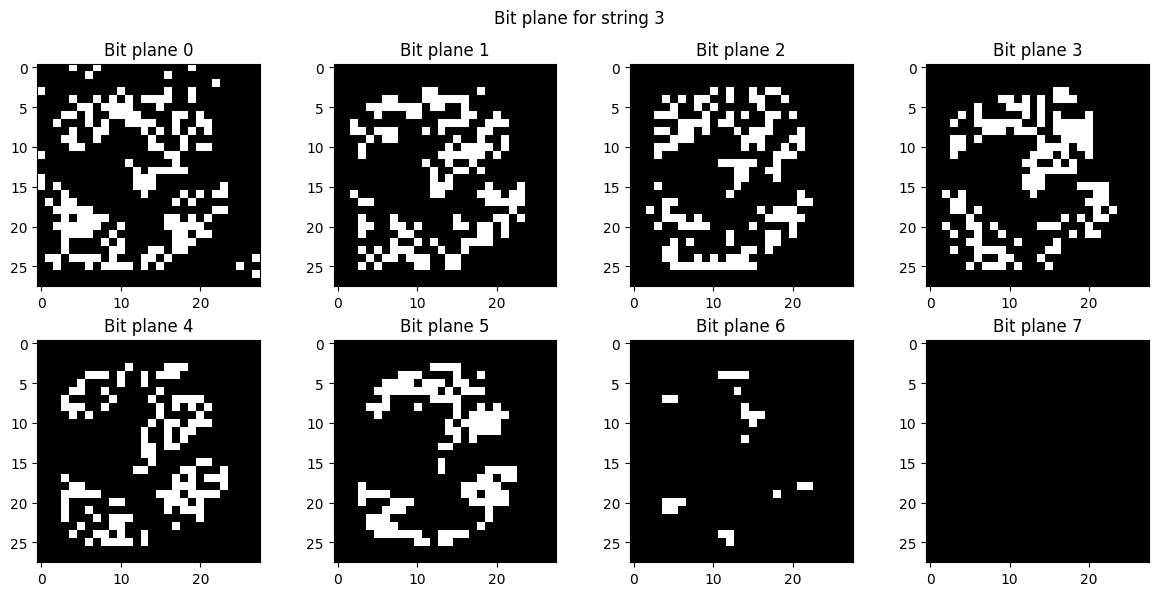
\includegraphics[width = 0.85\textwidth]{pics/output.png} 
    \end{block}
\end{columns}
\end{frame}

%===============================================================================
\begin{frame}[t]
    \frametitle{Аппаратные затраты}
    \centering
    \begin{table}[h]
        \centering
        \caption{Аппаратные затраты для 5 битного представления коэффициентов}
        \begin{tabular}{|>{\raggedright\arraybackslash}p{4cm}|>{\centering\arraybackslash}p{2.5cm}|>{\centering\arraybackslash}p{2.5cm}|>{\centering\arraybackslash}p{2.5cm}|}
            \hline
            Тип блока & Использовано & Доступно & Соотношение, \% \\
            \hline
            LUT as logic & 2180 & 17600 & 12.39 \\
            \hline
            LUT as memory & 60 & 6000 & 1 \\
            \hline
            Flip Flop & 862 & 35200 & 2.45 \\
            \hline
            RAMB18  & 10 & 120 & 8.33 \\
            \hline
            DSP & 0 & 80 & 0 \\
            \hline
            BUFG & 1 & 32 & 3.13 \\
            \hline
        \end{tabular}
    \end{table}
\end{frame}

%===============================================================================
\begin{frame}[t]
\frametitle{Выводы}
\begin{itemize}
    \item Рассмотренный эксперимент на основе НС прямого распространения с
    полносвязным слоем показывает, что формат представление 
    весовых данных существенно влияет на точность определения 
    до 5 битной разрядности. Дальнейшее увеличение разрядности 
    не несет значительных изменений в точности.
    \item Предложенная структура НС показывает, что при увеличении
    разрядности наблюдается линейный рост в потреблении LUT и FF блоков FPGA.
\end{itemize}
\end{frame}

%===============================================================================
% \begin{frame}
%     % \printbibliography
% \end{frame}
 

%------------------------------------------------------------------------------------------

%===============================================================================
\end{document}